% ===================================================================================================
\chapter{Molecular Dynamics Simulations}
% ===================================================================================================

% ---------------------------------------------------------------------------------------------------
\section{Molecular Dynamics in General}
% ---------------------------------------------------------------------------------------------------
Molecular dynamics (MD) as a simulation method originates from the 1950s and is therefore one of the oldest tools used in computational physics and materials research \cite{alder1957phase}.
On a fundamental level, MD consists of solving complex many-body problems iteratively to determine the forces acting on individual particles. These calculations, too complex  to utilize any analytical solution, are performed using numerical methods and allow us to relatively accurately simulate the dynamic evolution of (semi-)classical systems of particles. 

The basic algorithm of a MD simulation is described in fig. \ref{MD-schema}. The simulation is initiated by giving each atom, $i=1,...,N$, an initial position $\mathbf{r}_i^{(0)}$ and random velocity $\mathbf{v}_i^{(0)}$, consistent with the desired net temperature of the system. The positions and velocities of each particle are then updated by solving Newton's equations of motion
\begin{align}
\mathbf{F}_i(\mathbf{r}_i,t) = m_i\frac{d^2\mathbf{r}_i}{dt^2} = m_i\mathbf{a}_i(t) = -\nabla_{r_i}V(\mathbf{r}_i)
\end{align}
where $m_i$ is the mass of atom i, positioned at $\mathbf{r}_i$. The force $\mathbf{F}_i$ acting on each particle is determined by the interatomic potential $V(\mathbf{r}_i)$ and can be used to calculate the acceleration of each particle. The new positions and velocities are then simply functions of the acceleration and the simulation time step $\Delta t$. The simulation then proceeds through repeated evaluations of the equations of motion, updating the system in increments of $\Delta t$ time units. In order to avoid catastrophic errors in the conservation of energy, the time step must be shorter than the inverse vibrational frequency of any process in the system, typically around 1 fs. 

% [Periodic boundaries]


% [Thermostats, barostats]



% --------------- MD schematic ------------------------------------------------------------------------------------
\begin{figure}
\begin{center}
% Define block styles
\tikzset{
decision/.style = {diamond, draw, fill=green!40, 
    text width=4.5em, text badly centered, node distance=3cm, inner sep=0pt},
block/.style = {rectangle, draw, fill=cyan!30, 
    text width=20em, text centered, rounded corners, minimum height=2em},
cloud/.style = {draw, ellipse,fill=red!20, node distance=3cm,
    minimum height=2em}
    }

\begingroup  % compress equations
\medmuskip=2mu
\thinmuskip=1mu
\thickmuskip=2mu
\begin{tikzpicture}
\matrix (m)[matrix of nodes, column  sep=1.5cm,row  sep=5mm, align=center, nodes={rectangle,draw, anchor=center} ]{
    |[block]| {Set initial conditions $\mathbf{r}_i(t_0)$ and $\mathbf{v}_i(t_0)$, set a timestep $dt$ and reset $\mathbf{a}=0$, $_0t=0$}              &  \\
    %|[block]| {\textit{Estimation step:}\\ Estimate new atom positions; \\
    %  Move atoms: $\mathbf{r}_i^{(e)} = \mathbf{r}_i^{(j)} + \mathbf{v}^{(j)}dt + \mathbf{a}\frac{1}{2}dt^2 + ...$\\
    %  Update velocities: $\mathbf{v}^{(e)}=\mathbf{v}^{(f)}+\mathbf{a}dt + ...$}              &  \\
   |[block]| {Calculate $\mathbf{F}_i = -\mathbf{\nabla} V(\mathbf{r}_i)$ and $\mathbf{a}_i=\mathbf{F}_i/m_i$}              &  \\
   |[block]| {Adjust atom positions based on the new $\mathbf{a}_i$;\\
     Move atoms: $\mathbf{r}_i(t_{n+1}) = \mathbf{r}_i(t_n) + f(\mathbf{a}_i,\Delta t)$\\
      Update velocities: $\mathbf{v}(t_{n+1})=\mathbf{v}(t_n)+g(\mathbf{a}_i,\Delta t)$}              &  \\
   |[block]| {Apply boundary conditions, thermostats and barostats as needed}              &  \\
   |[block]| {Calculate and output physical quantities of interest}              &  \\
   |[block]| {$t_{n+1} = t_n+\Delta t$}              &  \\
   |[decision]| {End condition reached?}              &  \\
   |[block]| {Collect data and quit}              &  \\
};
\path [>=latex,->] (m-1-1) edge (m-2-1);
\path [>=latex,->] (m-2-1) edge (m-3-1);
\path [>=latex,->] (m-3-1) edge (m-4-1);
\path [>=latex,->] (m-4-1) edge (m-5-1);
\path [>=latex,->] (m-5-1) edge (m-6-1);
\path [>=latex,->] (m-6-1) edge (m-7-1);
%\path [>=latex,->] (m-7-1) edge (m-8-1);
\draw [>=latex,->] (m-7-1.west) -- node[above] {no} ++(-4,0cm) |- (m-2-1.west);
\draw [>=latex,->] (m-7-1.south) -- node[right] {yes}(m-8-1);
\end{tikzpicture}
\endgroup
\caption{A flowchart representation of a typical Molecular Dynamics simulation. Above, $f$ and $g$ refer to two different functions of the timestep and the acceleration. In the most simple case these would be $f(\mathbf{a}_i,\Delta t) = \mathbf{v}_i\Delta t + \mathbf{a}_i\Delta t^2$ and $g(\mathbf{a}_i,\Delta t) = \mathbf{a}_i\Delta t$, respectively.} 
\label{MD-schema}
\end{center}
\end{figure}
%------------------------------------------------------------------------------------------------------------------


\subsection{Interatomic potentials}

In an MD simulation, potential energies of simulated particles are calculated using so called interatomic potentials - mathematical functions designed to approximately emulate the interactions between atoms. These potentials are usually based upon the Born-Oppenheimer model, i.e. the electrons of alla atoms are permanently in the ground state and all interactions depend purely on the interatomic distance \cite{born1927quantentheorie}. In general terms, the potential energy of an atomistic system can be written as
\begin{align}
V_{tot} = \sum_i^N V_1(\mathbf{r}_i) + \sum_{i,j}^N V_2(\mathbf{r}_i, \mathbf{r}_j) +  \sum_{i,j,k}^N V_3(\mathbf{r}_i, \mathbf{r}_j, \mathbf{r}_k) + ...
\label{V_tot-ekv}
\end{align}
where $N$ is the number of atoms in the system and $V_1$, $V_2$ and $V_3$ respectively are one, two and three body terms \cite{potentialsTheory}.

The indices $i$, $j$ and $k$ iterate through the atom positions in three spatial dimensions and can be restricted to $i < j$ and $j < k$ for symmetric interactions such as monoelemental systems. The first term of eq. (\ref{V_tot-ekv}) can be discarded for systems not affected by an external field, an we are thus left with
\begin{align}
V_{tot} = \sum_i \sum_{j>i} V_2(\mathbf{r}_i, \mathbf{r}_j) + \sum_i \sum_{j>i} \sum_{k > j} V_3(\mathbf{r}_i, \mathbf{r}_j, \mathbf{r}_k) + ...
\end{align}
Potentials employing terms of a higher order than two are referred to as many-body potentials, while those using only the two first terms are pair potentials.

The atomic structure of metals allows the to be described particularly well using the so called Embedded Atom Method (EAM) formalism, giving the potential energy in the form
\begin{align}
V_{tot} = \sum_i^N F_i\, \bigg( \sum_j \rho\, (\mathbf{r}_{ij}) \bigg) + \frac{1}{2} \sum^N_{ij} V_2 (\mathbf{r}_{ij})
\end{align}
where  $F_i$ is a function of the summed electron density $\rho (\mathbf{r}_{ij})$ and $\mathbf{r}_{ij}$ denotes the distance $| \mathbf{r}_i - \mathbf{r}_j |$ between the $i$th and $j$th atoms. \cite{EAMmodel,dudarevEAMpotential}. 

For covalently bonded materials, is is often more accurate to use a Bond Order Potential (BOP), generally presented as
\begin{align}
V_{ij}(r_{ij}) =bV_{ijk}V_{\rm attractive}(r_{ij}) V_ {\rm repulsive}
\end{align}
Examples of BOPs are potentials of Tersoff, Brenner and Finnis-Sinclair type. \cite{tersoff1988new, brenner1990empirical, finnis1984simple} Both BOP and EAM potentials have the functional shape of a typical pair-potential, but act as many-body potentials due to many-body interactions embedded into the pair-terms.


% ---------------------------------------------------------------------------------------------------
\section{Molecular Dynamics for Simulating Isotope Exchange}
% ---------------------------------------------------------------------------------------------------
% [A few words about LAMMPS ]
% Large-scale Atomic/Molecular Massively Parallel Simulator (LAMMPS) \cite{lammpsMD}, 

The interatomic potential of choice for most of our simulations was the W-H-He EAM potential developed by Bonny \textit{et al.} and referred to as 'EAM1' in \cite{bonny2014binding}. The W-W interaction part of this potential is the same as 'EAM2' developed by Marinica \textit{et al.} in \cite{marinica2013interatomic} and well-known for providing elastic constants and point defect, dislocation and grain boundary properties in good agreement with Density Functional Theory (DFT) calculations and experiments \cite{bonny2014many}. The W-H-He potential, referred hereafter to as just 'EAM1', has been shown to relatively accurately recreate the interactions of H with both point defects and dislocations in W \cite{bonny2014binding, grigorev2015interaction}. 


% ===================================================================================================
\chapter{Simulation Setups}
% ===================================================================================================
We have studied isotope exchange in four common crytsallographic defect systems in tungsten. Regardless of the simulated defect, each simulation followed the same general pattern. First, a simulation cell of bulk W containing the defect was created and allowed to reach a minimum energy configuration by first using numerical minimization and then relaxation through repeatedly heating and cooling the system during short MD cycles. The method of energy minimzation used in all simulations is a Polak-Ribi\`{e}re conjugate gradient algorithm \cite{polak1969note}, used to iteratively adjust atom coordinates until a local energy minimum was found. 

After the initial relaxation, the defect was saturated with T during a 10...200 ns MD run and the excess was removed, prior to adding H to random TIS positions around the bulk material. Isotope exchange is then simulated by running MD for a total simulation time of 100...1450 ns. Periodic boundaries are applied in all directions and the pressure and temperature are controlled using a Nos\'{e}-Hoover thermostat and barostat, emulating an isothermal-isobaric ensemble. In a real world situation, a T atom leaving a defect and diffusing far away will very unlikely return to the same defect, instead of getting caught in another defect or leaving the material through a surface. Due to the periodic boundaries, however, this behavior is not seen as the T atom exiting the cell simply returns from the opposite side. T counter this, the simulation is performed in intervals of 5 ps (5000 time steps) and between each interval, any T atoms having moved 'far away' are removed from the simulation. This decision is made based on the current distance of each T atom from its initial position. If the distance exceeds a threshold of $d_{\rm{rmv}} =$ 14 \AA, i.e. ca 4.5 unit cells, the T atom is considered to have left the system. 




% --------------- IsoEx MD ------------------------------------------------------------------------------------
\begin{figure}
\begin{center}
% Define block styles
\tikzset{
decision/.style = {diamond, draw, fill=green!40, 
    text width=4.5em, text badly centered, node distance=3cm, inner sep=0pt},
block/.style = {rectangle, draw, fill=cyan!30, 
    text width=12em, text centered, rounded corners, minimum height=2em},
smallblock/.style = {block, text width=5em},
cloud/.style = {draw, ellipse,fill=red!20, node distance=3cm,
    minimum height=2em}
    }
\begingroup  % compress equations
\medmuskip=2mu
\thinmuskip=1mu
\thickmuskip=2mu
\begin{tikzpicture}
\matrix (m)[matrix of nodes, column  sep=0.0cm,row  sep=5mm, align=center, nodes={rectangle,draw, anchor=south} ]{
   |[block] (initI)| {Create simulation cell containing defect} & \\
   |[block] (initII)| {Relax \& add hydrogen} & \\
    |[block] (MD)| {Run MD for 5000 time steps}          &  \\
    |[block] (Calcd)| {Calculate $d_i$}          &  \\
   |[decision] (IsOut)| {$d_i > d_{\rm{rmv}}$?}              &  \\
       & |[smallblock] (Rmv)| {Remove $i$th T atom}         &  \\
   |[decision] (IsEnd)| {End condition reached?}              &  \\
   |[block] (End)| {Save results \& quit}   & \\
};
\path [>=latex,->] (initI) edge (initII);
\path [>=latex,->] (initII) edge (MD);
\path [>=latex,->] (MD) edge (Calcd);
\path [>=latex,->] (Calcd) edge (IsOut);
\draw [>=latex,->] (IsOut.east) -| node[above, near start] {yes} (Rmv.north);
\draw [>=latex,->] (IsOut.south) -- node[right] {no}(IsEnd);
\draw [>=latex,->] (Rmv.south) |- (IsEnd.north);
\draw [>=latex,->] (IsEnd.west) -- node[above] {no} ++(-2,0cm) |- (MD.west);
\draw [>=latex,->] (IsEnd.south) -- node[right] {yes}(End);
\end{tikzpicture}
\endgroup
\caption{A flowchart representation of the isotope exchange simulations. Variable $d_i$ refers to the distance between current and initial point of T atom $i$.} 
\label{Fig:isoExSimus}
\end{center}
\end{figure}


% ---------------------------------------------------------------------------------------------------
\section{Vacanies}
% ---------------------------------------------------------------------------------------------------
In the vacancy case, a monovacancy was created by removing the middlemost W atom of a $10\times 10 \times 10$ unit cell (2000 atom) W lattice. As seen in fig. \ref{Fig:monovac_system}, six T atoms were then added to the vacancy at their lowest energy positions \cite{heinola2010hydrogen}, i.e. at the octahedral interstitial sites, forming a square bipyramid. A total of 19 H atoms were then deposited to randomly chose tetragonal interstitial sites around the simulation W lattice, bringing the (H+T)/W ratio to 0.0125. The T/H ratio, on the other hand, is 0.32.

A divacancy system was constructed similarly by instead removing two neighboring W atoms and adding 10 T atoms to the defect.

\begin{figure}[!ht]
\center
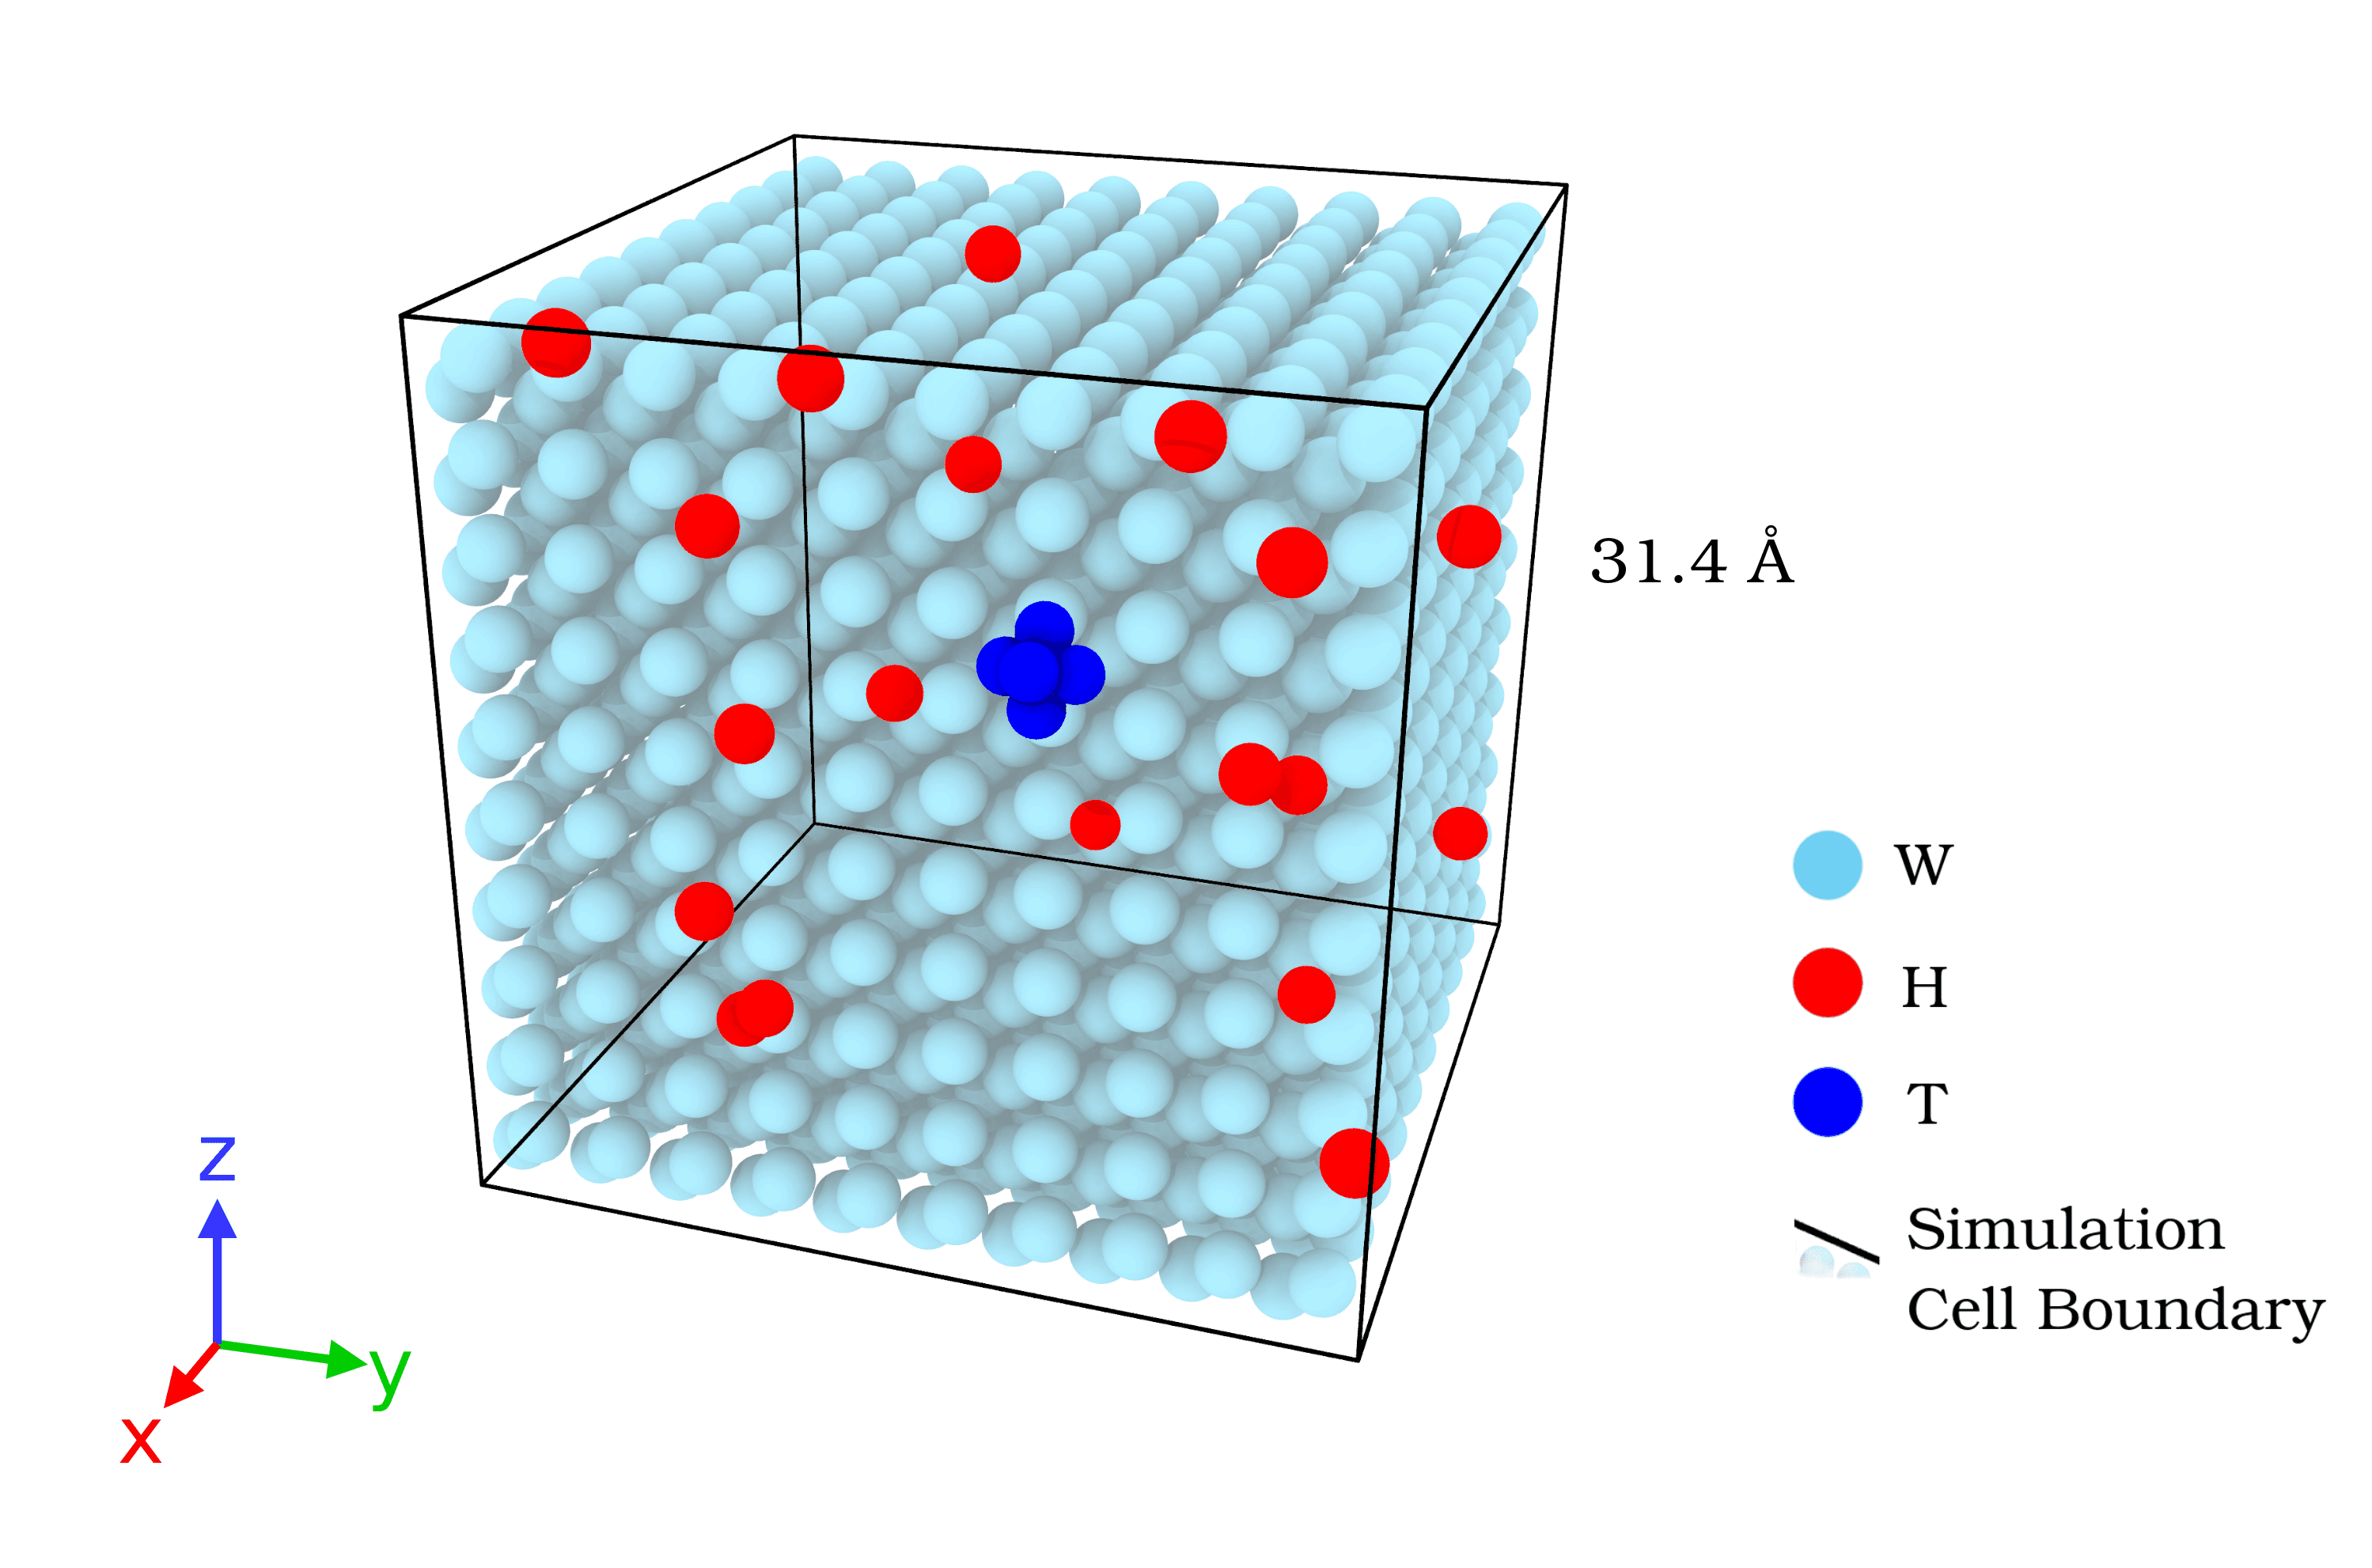
\includegraphics[scale=0.11]{1Vac_system.png}
\caption{The initial state of the simulation cell used in the monovacancy simulations. The W atoms are rendered translucent to display the positions of the hydrogen isotopes.}
\label{Fig:monovac_system}
\end{figure}

% ---------------------------------------------------------------------------------------------------
\section{Dislocations}
% ---------------------------------------------------------------------------------------------------
In the dislocation case, we have created a 1/2\hkl[1 1 1]\hkl{1 0 0} edge dislocation, in a $109.0 \times 136.8 \times 18.4$ $\AA^3$ tungsten super cell with the $x$, $y$ and $z$ axes oriented along the crystal directions  \hkl[1 1 1], \hkl[1 1 -2] and \hkl[-1 1 0] respectively. The supercell was then divided into three equally thick slices, parallel to the $xz$ plane and a dislocation introduced through the addition of a \hkl{1 1 1} atom plane (parallel to the $yz$ plane) from to the middlemost slice. In order to facilitate the formation of a natural dislocation and to enable the use of periodical boundary conditions, the atom positions in the middle slice were finally compressed slightly.

% [Skiss of the dislocation manufacturing process?]

\begin{figure}[!ht]
\center
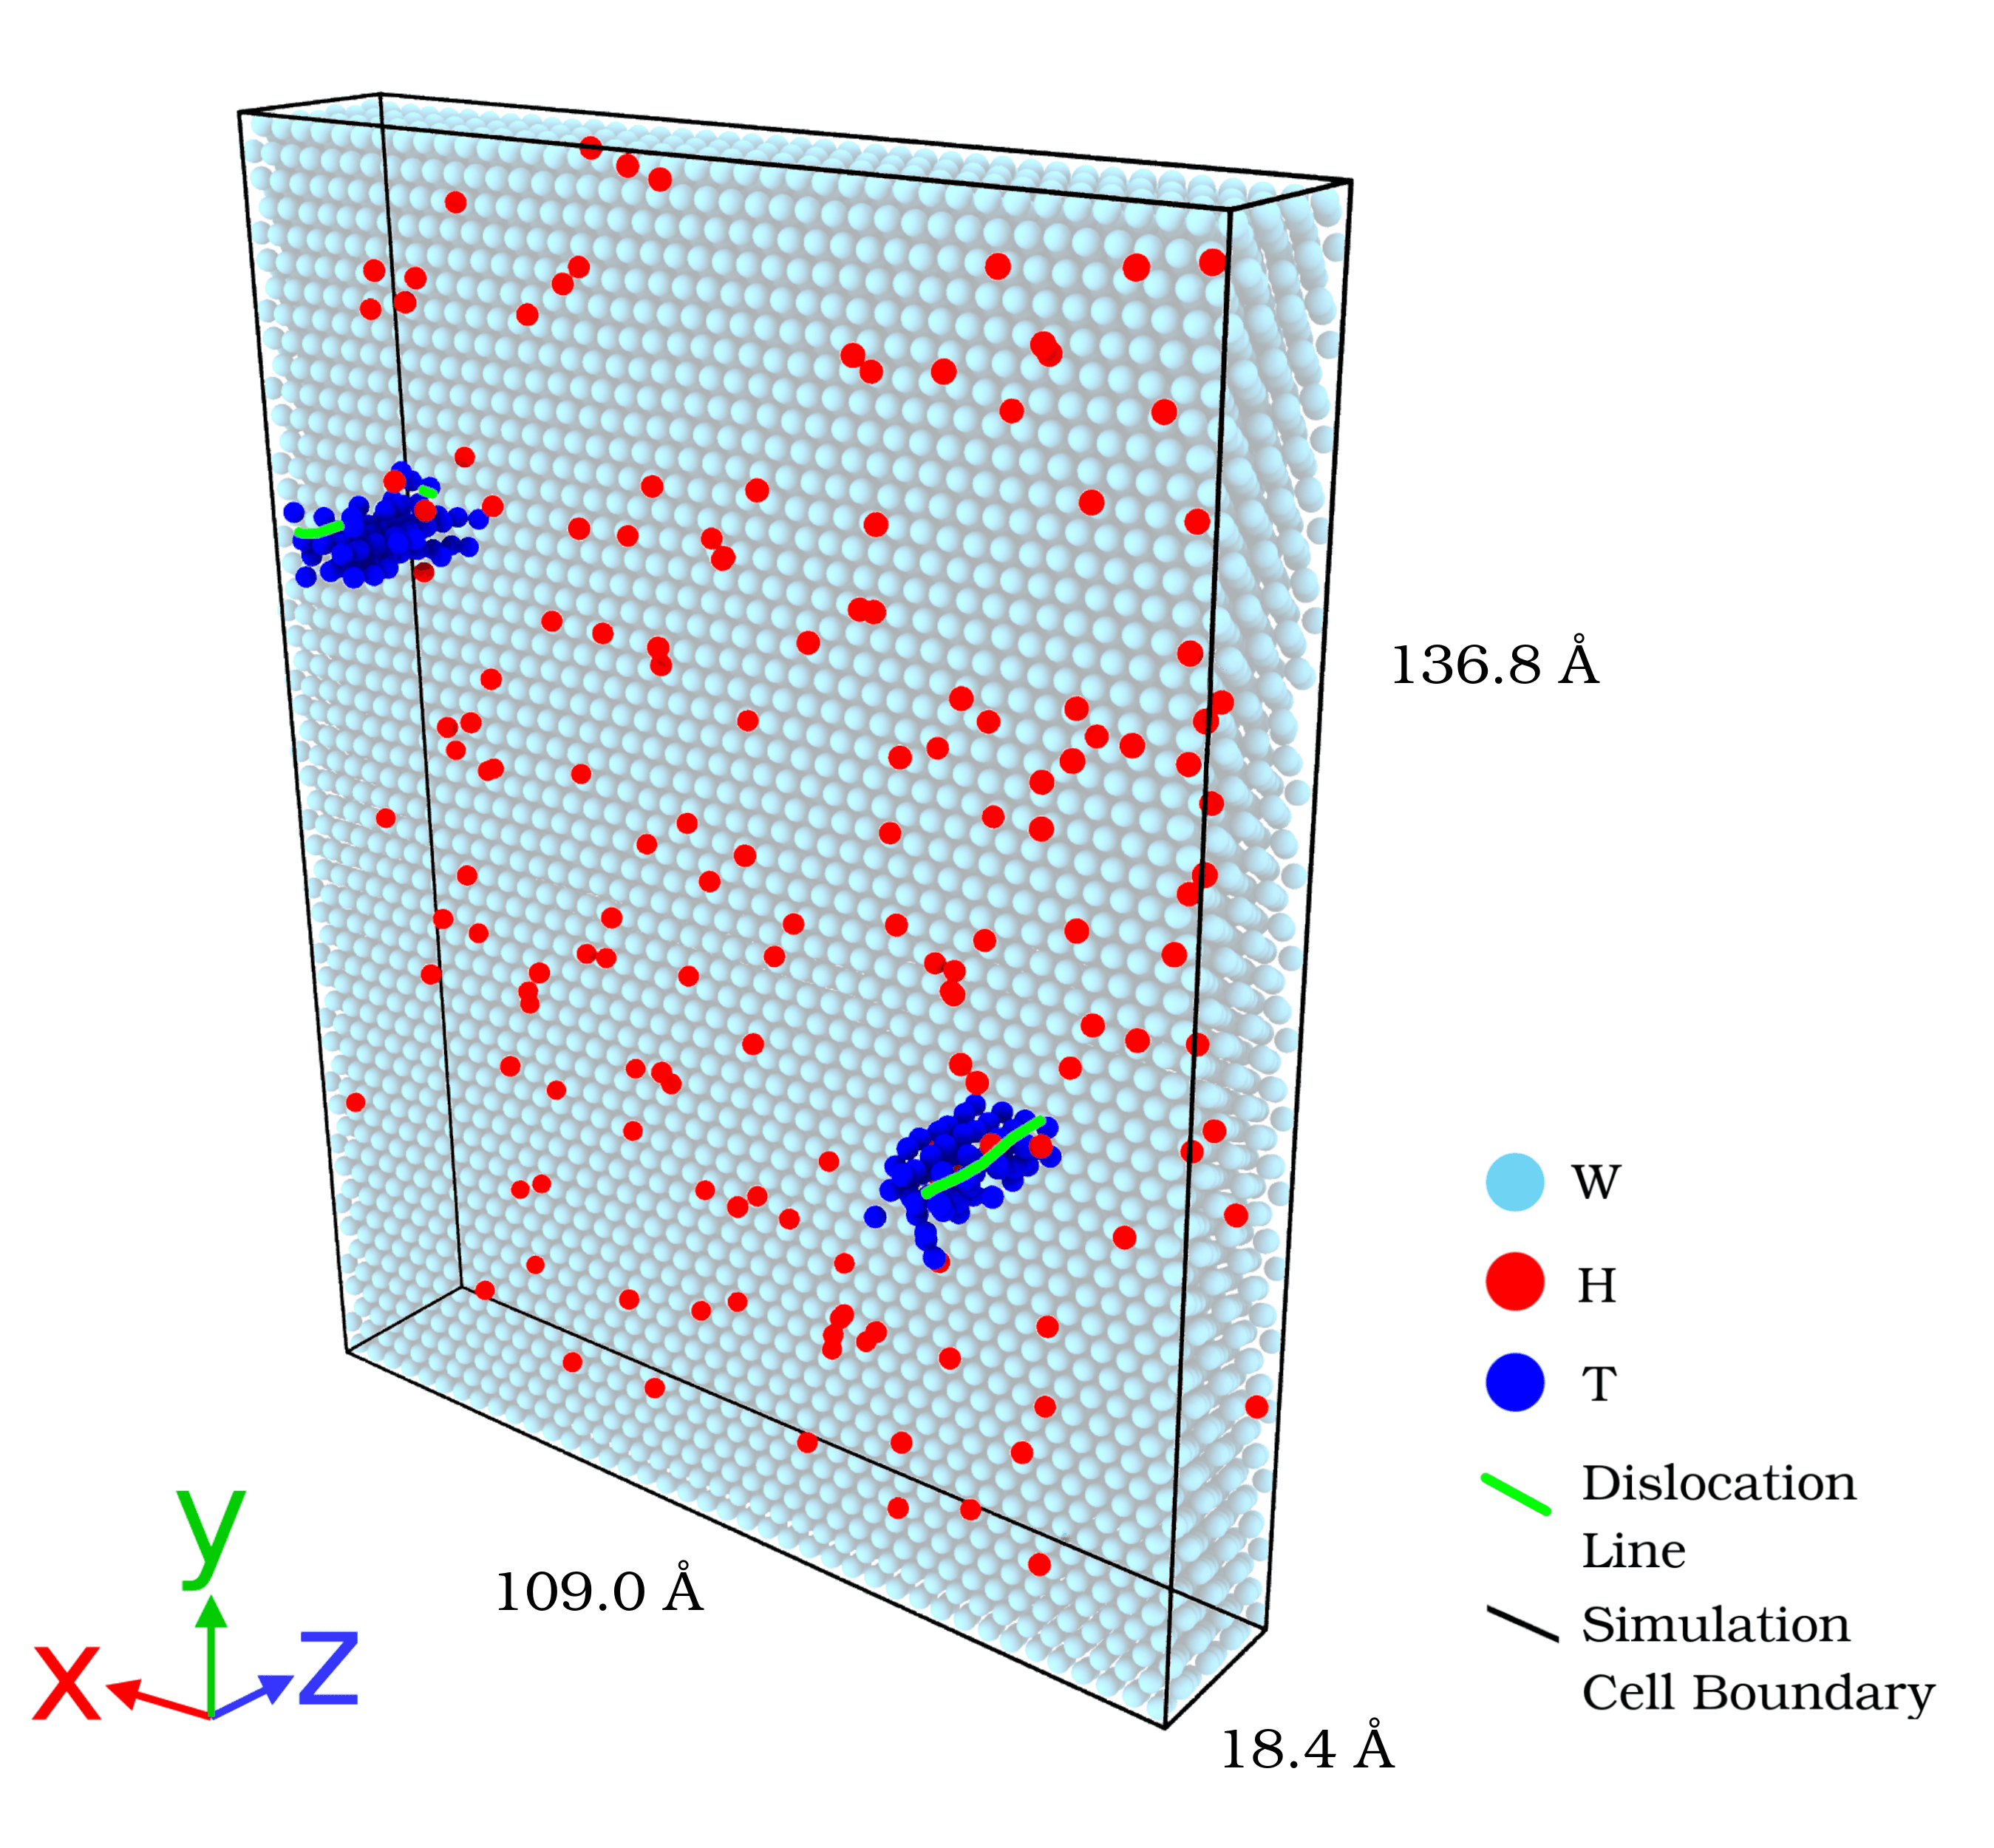
\includegraphics[scale=0.11]{disloc_system.png}
\caption{The initial state of the simulation cell used in the dislocation simulations. The W atoms are rendered translucent to display the positions of the hydrogen isotopes. The dislocation, together with its periodic images, is visualized using a defect mesh.}
\label{Fig:disloc_system}
\end{figure}

% ---------------------------------------------------------------------------------------------------
\section{Grain Boundaries}
% ---------------------------------------------------------------------------------------------------
% $\Sigma$5\hkl{310}/\hkl[001]
A simulation cell containing a \hkl{310}\hkl[001] tilt grain boundary was created by growing together two separate tungsten lattices, each rotated through $\pm18.43^\circ$ respectively, around the $z$-axis. The $x$-axes of the lattices now point along directions of \hkl<310>, we have a system which has a periodicity of $\sqrt{10}~a$ along the $x$- and $y$-axes, and $a$ along the $z$-axis. In order to minimize the number of atoms needed to simulate the system we can set $y >> x \approx z$ and again use periodic boundaries.

% Zhou_2009_H_behaviour_in_W_grain_boudnary_FP.pdf

\begin{figure}[!ht]
\center
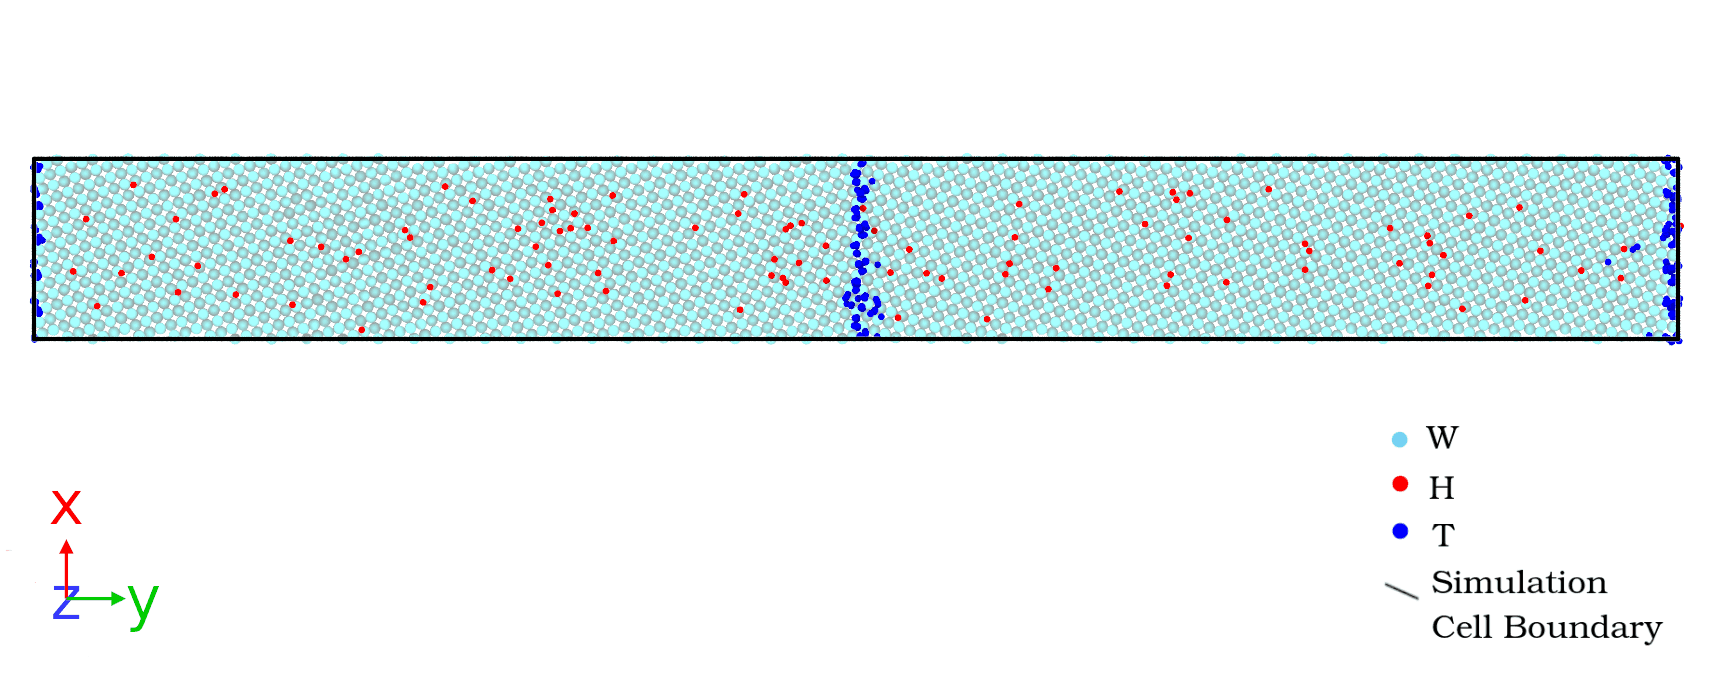
\includegraphics[scale=0.22]{GB_system.png}
\caption{The initial state of the simulation cell used in the grain boundary simulations. The W atoms are rendered translucent to display the positions of the hydrogen isotopes.}
\label{Fig:GB_system}
\end{figure}

% ---------------------------------------------------------------------------------------------------
%\section{Impurities}
% ---------------------------------------------------------------------------------------------------
